\documentclass[a4paper]{article}

%% Language and font encodings
\usepackage[english]{babel}
\usepackage[utf8x]{inputenc}
\usepackage[T1]{fontenc}

%% Sets page size and margins
\usepackage[a4paper,top=3cm,bottom=2cm,left=4cm,right=4cm,marginparwidth=1.75cm]{geometry}

%% Useful packages
\usepackage{amsmath}
\usepackage{graphicx}
\usepackage[colorinlistoftodos]{todonotes}
\usepackage[colorlinks=true, allcolors=blue]{hyperref}
\usepackage{amssymb} %for writing Real number symbol 
\numberwithin{equation}{section}
\usepackage{color,soul}
\usepackage{float}


\DeclareMathOperator*{\argmin}{argmin} 

\newcommand{\minim}[2]{\begin{equation}
\begin{aligned}
&\text{minimize}& &#1\\
&\text{subject to}& &#2
\end{aligned}
\end{equation}}

\newcommand{\minimlabel}[3]{\begin{equation}
	\begin{aligned} 
	&\text{minimize}& &#1\\
	&\text{subject to}& &#2
	\end{aligned}\label{eq:#3}
	\end{equation}}

\newcommand{\maxim}[2]{\begin{equation}
\begin{aligned}
&\text{maximize}& &#1\\
&\text{subject to}& &#2
\end{aligned}
\end{equation}}

\newcommand{\maximall}[3]{\begin{equation}
\begin{aligned}
&\text{maximize}& &#1\\
&\text{subject to}& &#2 \\
& & &#3
\end{aligned}
\end{equation}}

\newcommand{\minimall}[3]{\begin{equation}
\begin{aligned}
&\text{minimize}& &#1\\
&\text{subject to}& &#2\\
& & &#3
\end{aligned}
\end{equation}}





\title{Inverse Covariance Selection via ADMM}
\author{Arturo Arranz Mateo}

\begin{document}
\maketitle

\begin{abstract}
In a Gaussian distributions, conditional independence between variables correspond to zero entries in the inverse covariance matrix. However, estimating the inverse from samples under the assumption of sparsity is not straight forward. For small matrices an fixed sparse pattern, it can be calculated as a convex optimization problem. Nonetheless, for high dimensional data and general sparse patterns the problem becomes intractable and heuristics are needed, such as lasso regularization. Another associated problem of with high dimensional data, which accounts for most of the data applications nowadays, is the problem of storage and computation time. In this project explore the distributed algorithm, Alternating Directions Method of Multipliers(ADMM) for the \textit{inverse covariance selection problem} thanks to its decomposability nature and finally we show some applications for political voting analysis in the US senate. 
\end{abstract}

\section{Alternating Direction Method of Multipliers}

The main foundations of ADMM are \textit{the dual ascent method} for solving convex optimization problems, \textit{dual decomposition} for decomposing the objective and constraint functions and \textit{the method of multipliers} which guarantee differentiability under mild conditions.

\subsection{Dual Ascent}

Given the following convex optimization problem with linear constraints,
\minimlabel{f(x)}{Ax=b}{original}
with variables $x \in \mathbb{R}^n$, where $A \in \mathbb{R}^{m\times n}$, and $f: \mathbb{R}^n \rightarrow \mathbb{R}$ is convex. The lagrangian,
\begin{equation*}
	L(x,y)=f(x) + y^T(Ax-b)
\end{equation*}
and the dual function,
\begin{equation*}
	g(y) = \inf_x L(x,y) = -f*(-A^Ty)-b^Ty
\end{equation*}
where $y \in \mathbb{R}^m$ is the Lagrangian multiplier, and $f^*$ is the convex conjugate of f. The dual problem then becomes 
\begin{equation*}
	\mbox{minimize} \quad g(y)
\end{equation*}
if strong duality holds, then we can recover the solution of the primal problem,$x^*$ from the the dual problem solution, $y^*$ as
\begin{equation*}
	x^* := minimize L(x,y^*)
\end{equation*}
the \textit{dual ascent method} consists on taking steps towards the dual function gradient and updating the primal solution iteratively,

\begin{align}
&x^{k+1} := \argmin_x L(x,y^k) \label{eq:updual1}\\ 
&y^{k+1} := y^k + \alpha^k(Ax^{k+1}-b) \label{dual2}
\end{align}
where $\alpha^k>0$ is the step size, which control how fast the solution converges, but in case of too high value it might lead to convergence problems. The names \textit{dual ascent} comes from the fact that $g(y)$ increases in every step. However, some conditions must hold to guarantee convergence and functioning of the algorithm. For instance, $g(y)$ must be differentiable in order to evaluate the it gradient, and \textit{dual subgradient method} should be used instead. Another exampel is the case when $f(x)$ is a non-zero affine function, in which case the update (\ref{eq:updual1}) would fail since the Lagrangian is unbounded below for most of $y$ and $x$.

\subsection{Dual decomposition}

The strength of \textit{dual ascent} is that it can lead to a decentralized algorithm when the objective and constraint functions are separable,

\begin{equation*}
f(x) = \sum_{i=1}^{N}f_i(x_i) \qquad Ax = \sum_{i=1}^{N}A_ix_i 
\end{equation*}
where $x = (x_1,x_2,...x_N)$ and $x_i \in \mathbb{R}^{n_i}$. Then the Lagrangian looks like

\begin{equation*}
	L(x,y) = \sum_{i=1}^{N}f_i(x_i)+y^T(A_ix_i - b) -(1/N)y^Tb
\end{equation*}
meaning that the dual ascent method consist in N primal variables updates and one dual step as

\begin{align}
	&x_i^{k+1} := \argmin_x \quad L_i(x_i,y^k)\\
	&y^{k+1} := y^k + \alpha^k(Ax^{k+1} - b)
\end{align}

\subsection{Method of multipliers}

As already stated, dual ascent assume very strict conditions on the initial problem such as strict convexity and finiteness of $f$. In order to overcome some of this issues the \textit{augmented Lagrangian} is introduced,

\begin{equation*}
	L_\rho(x,y) = f(x) + y^T(Ax-b) + (\rho/2)||Ax-b||_2^2
\end{equation*}
where $\rho$ is the \textit{penalty parameter}. The \textit{augmented Lagrangian} is equivalent to solve the transformed initial problem 

\minimlabel{f(x)+||Ax-b||_2^2}{Ax=b}{trans_prob}
The problem (\ref{eq:trans_prob}) is clearly equivalent to the original problem, (\ref{eq:original}), since the residual $Ax -b$ is zero at the optimal feasible point. This new formulation brings the benefit of differentiability under rather mild conditions on the original problem. The new dual functions is $g_\rho(y)=inf L_\rho(x,y)$. This leads to the \textit{method of multipliers}

\begin{align}
	&x^{k+1} :=\argmin_x \quad L_\rho(x,y^k)\label{eq:mmstep1}\\ 
	&y^{k+1} = y^k + \rho(Ax^{k+1}-b)		
\end{align}
In practice the learning parameter could be anything, instead of $\rho$, but it is motivated for convergence reasons. The original problem posses the following primal and dual feasibility conditions

\begin{equation*}
	Ax^* -b =0, \qquad \nabla f(x^*) + A^Ty^* = 0,
\end{equation*}
Now, if we look at the minimization step (\ref{eq:mmstep1}) it minimize the augmented Lagrangian,$L_\rho(x,y^k)$

\begin{align*}
	0 &=\nabla_xL(x^{k+1},y^k)\\
	&= \nabla_x f(x) + y^TA + \rho(Ax^{k+1} -b)\\
	&= \nabla_x f(x^{k+1}) + A^Ty^{k+1}
\end{align*}
making every step dual feasible. However the method of multipliers has a drawback. Even thought that $f$ is separable, its augmented Lagrangian, $L_\rho$, is not. This problem is addressed by the Alternating Direction Method of Multipliers

\subsection{ADMM algorithm}

ADMM mix the decomposability of dual ascent with the superior convergence properties of \textit{method of multipliers}. Given a problem as 

\minimlabel{f(x)+g(z)}{Ax+Bz=c}{twovariables}
The associated augmented Lagrangian would be,

\begin{equation*}
	L_\rho(x,z,y) = f(x)+g(z)+y^T(Ax + Bz-c)+(\rho/2)||Ax+Bz-c||_2^2
\end{equation*}
If we would intended to apply \textit{the method of multipliers} the iteration updates would look like,

\begin{align*}
	&(x^{k+1},z^{k+1}) := \argmin_x L_\rho(x,z,y^k)\\
	&y^{k+1} := y^k + \rho(Ax^{k+1}+Bz^{k+1} -c)
\end{align*}
where $x$ and $z$ are jointly optimized. However we an take an additional step and optimize each of the variables separately.

\begin{align}
&x^{k+1} := \argmin_x \quad L_\rho(x,z^k,y^k)\\
&z^{k+1} := \argmin_z \quad L_\rho(x^{k+1},z,y^k)\\
&y^{k+1} := y^k + \rho(Ax^{k+1}+Bz^{k+1} -c)
\end{align}
this is \textit{finally} the \textit{Alternating Direction Method of Multipliers}. The \textit{alternating} accounts for the fact that $x$ and $z$ can be minimized in an alternating or sequential fashion. 

\subsubsection{Scaled form}

The ADMM updates can be reformulated in a slightly different form which usually lead to shorter equations. If we define the residual as $r=Ax+Bz-c$ and $u = (1/\rho)y$ as the scaled dual variable, the augmented Lagrangian of the problem (\ref{eq:twovariables}) follows as

\begin{equation*}
	L_\rho(x,z,u) = f(x) + g(z) + (\rho/2)||r+u||_2^2 - (\rho/2)||u||_2^2
\end{equation*}
and then the \textit{scaled} form of ADMM 

\begin{align}
&x^{k+1} := \argmin_x \quad \Big(f(x)+(\rho/2)||Ax+Bz^k-c+u^k||_2^2\Big)\\
&z^{k+1} := \argmin_z \quad \Big(g(z)+(\rho/2)||Ax^{k+1}+Bz-c+u^k||_2^2\Big)\\
&y^{k+1} := y^k + \rho(Ax^{k+1}+Bz^{k+1} -c)
\end{align}

\subsubsection{Optimality conditions and Stopping criterion}
The optimality conditions for the problem \ref{eq:twovariables} are primal feasibility,
\begin{equation}
	Ax^* + B^*z -c = 0 \label{eq:primal_fes}
\end{equation}
and dual feasibility,
\begin{align}
	&0\in \partial f(x^*)+A^Ty^*\label{eq:dual_fes1}\\
	&0\in \partial g(z^*)+B^Ty^* \label{eq:dual_fes2}
\end{align}
for the same reasons as explained in the \textit{method of multipliers} the $z^{k+1}$ and $y^{k+1}$ always satisfy (\ref{eq:dual_fes2}) so we have to only look at (\ref{eq:dual_fes1}) and (\ref{eq:primal_fes}). Since $x^{k+1}$ minimize $L_\rho(x,z^k,y^k)$ by definition we have

\begin{align*}
	0 &\in \partial f(x^{k+1}) +A^Ty^k+\rho A^T(Ax^{k+1}+Bz^k-c)\\
	&=\partial  f(x^{k+1}) + A^T(y^k+\rho r^{k+1} \rho B(z^k - z^{k+1}))\\
	&=\partial f(x^{k+1}) + A^Ty^{k+1} \rho A^TB(z^k - z^{k+1})),\\	
	\rho A^TB(z^k - z^{k+1})&=\partial f(x^{k+1}) + A^Ty^{k+1})
\end{align*}
So we can define  

\begin{equation*}
	s^{k+1} = \rho A^TB(z^k - z^{k+1})
\end{equation*}
as the \textit{dual residual} for (\ref{eq:dual_fes1}) and $r^{k+1}=Ax^{k+1}+Bz^{k+1}-c$ as the \textit{primal residual} for (\ref{eq:primal_fes}).





\section{Inverse Covariance Selection}

Zero entries in the inverse covariance matrix correspond to conditional independence of random variables, i.e. knowing the value of one variable do not give information about other knowing the rest. Non-zero entries in the covariance matrix in the case of conditional independence might be contaminated by other variables correlations.

 Estimating the inverse covariance for small matrices and fixed sparse patterns is a tractable convex optimization problem. However, when a priori it is not known which variables are conditionally independent it becomes a combinatorial problem which scales exponentially with $n$. Lasso regularization is an heuristic which address this issue.

\subsection{Sparse regularization}
Suppose the case where we have samples from a zero mean Gaussian distribution,

\begin{equation*}
	x_i \sim \mathcal{N}(0,\Sigma), \quad i=1,2,...,N
\end{equation*}
which computational covariance matrix will be denoted as $C$. One way to estimate the inverse covariance is by means of the Kullback-Leibler divergence which is defined as 
\begin{equation*}
	D_{KL}(\mathcal{N}_1||\mathcal{N}_0) = \frac{1}{2}\Big(tr(\Sigma^{-1}_0\Sigma_1)+(\mu_0-\mu_1)^T\Sigma^{-1}_0 (\mu_0-\mu_1) -k +ln\Big(\frac{det\Sigma 0}{det \Sigma_1}\Big)\Big)
\end{equation*}
for two k-dimensional Gaussian distributions. So if we define $S = \Sigma^{-1}_1 $ and $X = \Sigma_0$ and minimize the $D_{KL}$ respect to X we have
\begin{equation}
	\mbox{minimize}\quad \textrm{Tr}(CX)-\textrm{lndet} X+ cte
\end{equation}
after assuming that both distributions have the same mean. Since the Kullback divergence is a measure on how similar two distributions are, after the minimization problem we would have $C = X^{-1}$. Therefore, $X$ is the inverse covariance estimation. 

Nonetheless what we are trying to estimate is a sparse general pattern on $X$ which can be introduced through Lasso regularization

\begin{equation}
\mbox{minimize}\quad \textrm{Tr}(CX)-\textrm{lndet} X+ \lambda |X|_1
\end{equation}

\subsection{ADMM formulation}

The same problem can be expressed as constrained optimization problem with two variables,

\minimlabel{\quad \textrm{Tr}(SX)-\textrm{lndet} X+ \lambda |Z|_1}{X-Z=0}{admm_problem}
now, following the ADMM framework it can be solved iteratively with the updates

\begin{align*}
&X^{k+1} := \argmin_x \quad\Big(\textrm{Tr}(CX)-\textrm{lndet}X+(\rho/2)||X-Z^k+U^k||_F^2\Big)\\
&Z^{k+1} := \argmin_z\quad \Big(\lambda||Z||_1+(\rho/2)||X-Z^k+U^k||_F^2\Big)\\
&U^{k+1} := U^k + X^{k+1}+Z{k+1}
\end{align*}
the updates can be simplify even further. For example the there exists a closed form solution for the z-minimization step which corresponds to a soft thresholding operation \cite[p.~23]{convexanalysis}

\begin{equation*}
	Z_{ij}^{k+1} = S_{\lambda/\rho}(X^{k+1}_{ij}+U^k_{ij})
\end{equation*}
but also the x-minimization step can be expressed as a closed from solution \cite[p.~47]{ADMM}

\begin{equation*}
X^{k+1} = Q\hat{X}Q^T
\end{equation*}
where $Q$ comes from the orthogonal eigenvalue decomposition of $\rho(Z^k-U^k)-S=Q\Lambda Q^T$ and $\hat{X}$ is a diagonal matrix with the form,

\begin{equation*}
	\hat{X}_{ii} = \frac{\lambda_i+\sqrt{\lambda_i^2+4\rho}}{2\rho}
\end{equation*}
which turns out to be a very cheap computational algorithm, where most of the effort is calculating an eigenvalue decomposition.


\subsubsection{Stopping criteria}

The algorithm is iterated until the primal and dual residuals

\begin{equation*}
R^{k+1} = X-Z \qquad S^{k+1} = \rho(Z^k-Z{k+1})
\end{equation*}
are less than the primal and dual tolerance

\begin{equation*}
\epsilon_{primal}>||R^{k+1}||_2 \qquad\epsilon_{dual} > ||S{k+1}||_2
\end{equation*}
where $\epsilon_{primal}$ and $\epsilon_{dual}$ are derived from the optimality conditions in the Annex

\begin{align}
	&\epsilon_{primal} = \epsilon_{abs}\sqrt{n}+ \epsilon_{rel}\max(||X||_2,||Z||_2) \label{eq:ep_primal}\\
	&\epsilon_{dual} = \epsilon_{abs}\sqrt{p}+ \epsilon_{rel}||S^T-X^{-T}+\rho U||_2 \label{eq:ep_dual}
\end{align}
where $\epsilon_{abs}$ and $\epsilon_{rel}$ are the absolute and relative tolerance for controlling accuracy of the solution. 







\section{Results}

Data from the US senate government \cite{voting} has been analyzed in order to find dependencies among politician during voting processes. The dataset consists on all the 2017 senate voting records which has 191 samples of 100 politicians stored in a vector $X \in \mathbb{R}^{100}$, where the first 46 entries are democrat members, the 2 following are independent senators and the rest 52 are republicans.

The computational covariance matrix has been fed to the ADMM algorithm for different regularization problems. In the figure \ref{fig:sparse} is represented the sparse pattern found for different values of $\lambda$, where white space means a zero entry. In one extreme, for $\lambda=0.3$ we see a diagonal matrix, where each politician vote completely independently. In the other extreme for $\lambda=0.001$ we see a dense inverse covariance matrix, where everyone depends on everyone else. However, for $\lambda=0.05$ and $0.01$ density is only present in first and fourth quadrant. This results suggest, as expected, that each politician vote depends on what their party fellows are voting. 

\begin{figure}[h]
	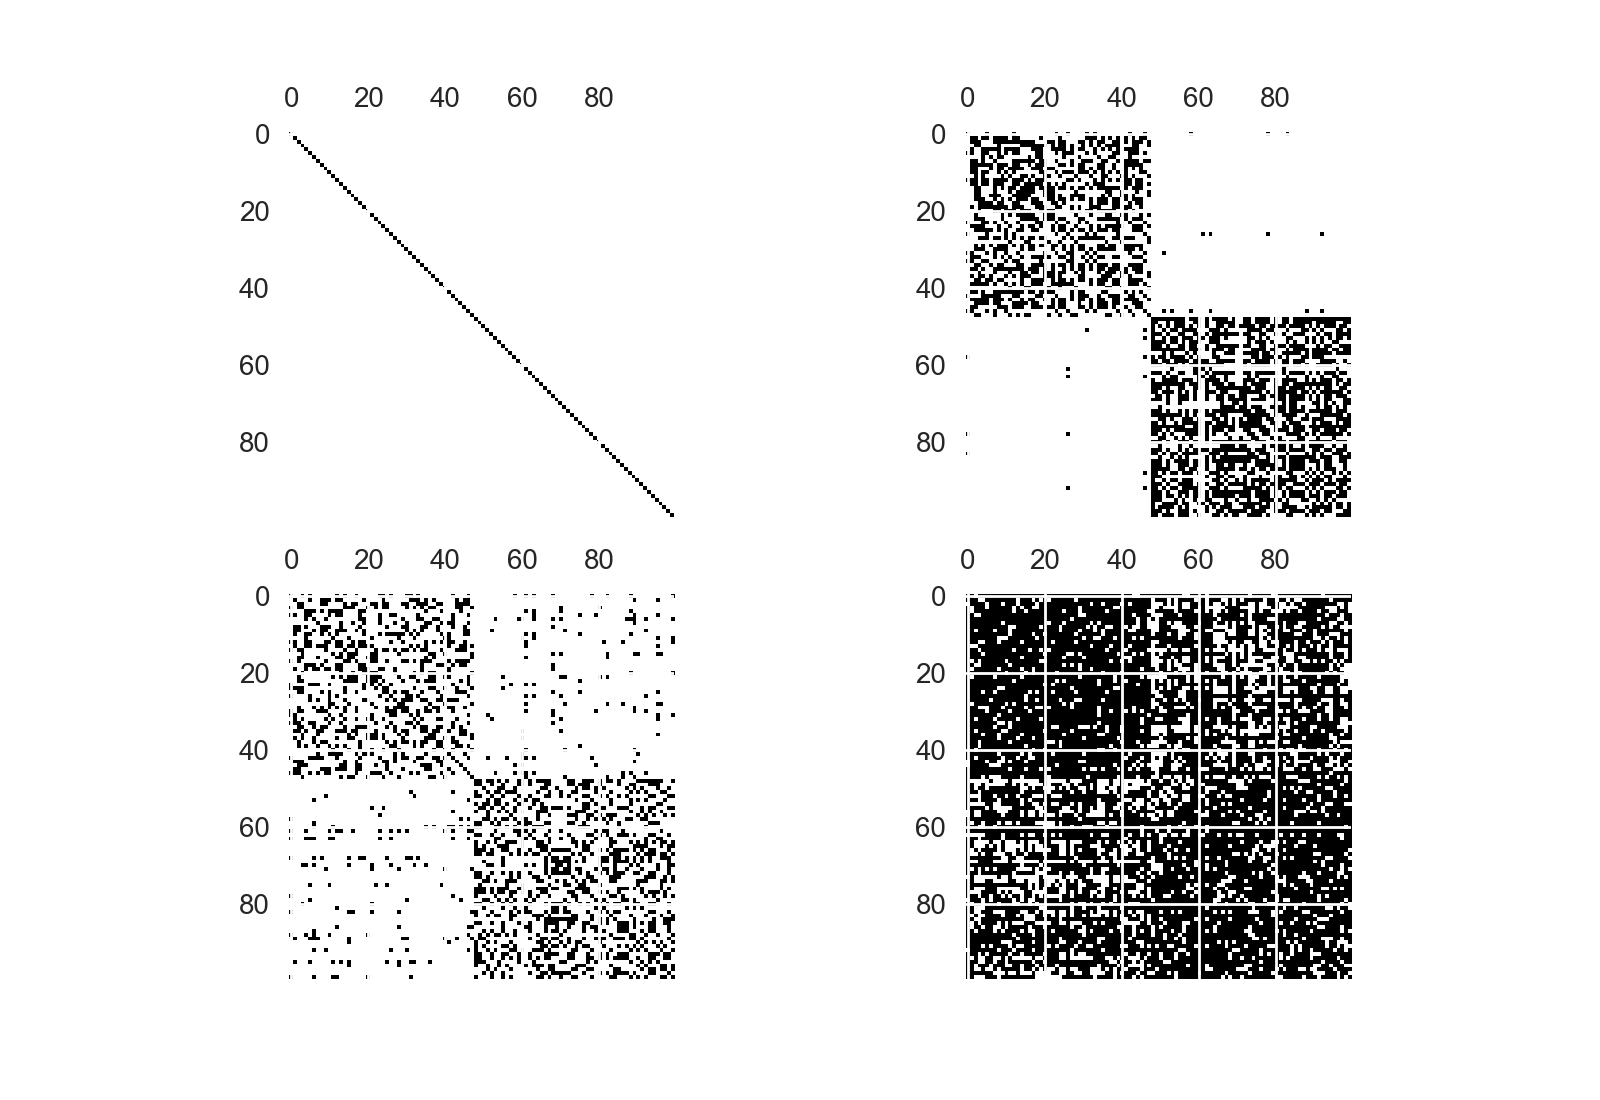
\includegraphics[width=1.1\textwidth]{figures/sparse_pattern.png}
	\caption{By order, sparse patterns for $\lambda$=0.3, 0.05, 0.01 and 0.001}
	\label{fig:sparse}
\end{figure}

The absolute and relative tolerance in (\ref{eq:ep_primal}) and (\ref{eq:ep_dual}) for all the experiments have been set to $10^{-3}$. The figure \ref{fig:convlambda} shows convergence of primal and dual residuals for different regularization values and fixed $\rho$. For $\lambda = 0.3$ it takes more time, since the relative tolerance is smaller, while for $\lambda = 0.001$ it takes longer since the residuals decrease slower.  
\begin{table}[h]
	\centering
	\begin{tabular}{l*{5}{c}r}
		Regularization($\lambda$)& 0.3 & 0.1 & 0.05 & 0.01 & 0.001 \\
		\hline
		Iterations & 224 & 47 & 40 & 96 & 152   \\
	\end{tabular}
	\label{tab:iterlambda}
	\caption{Number of iterations depending on $\lambda$}
\end{table}

\begin{figure}[H]
	\centering
	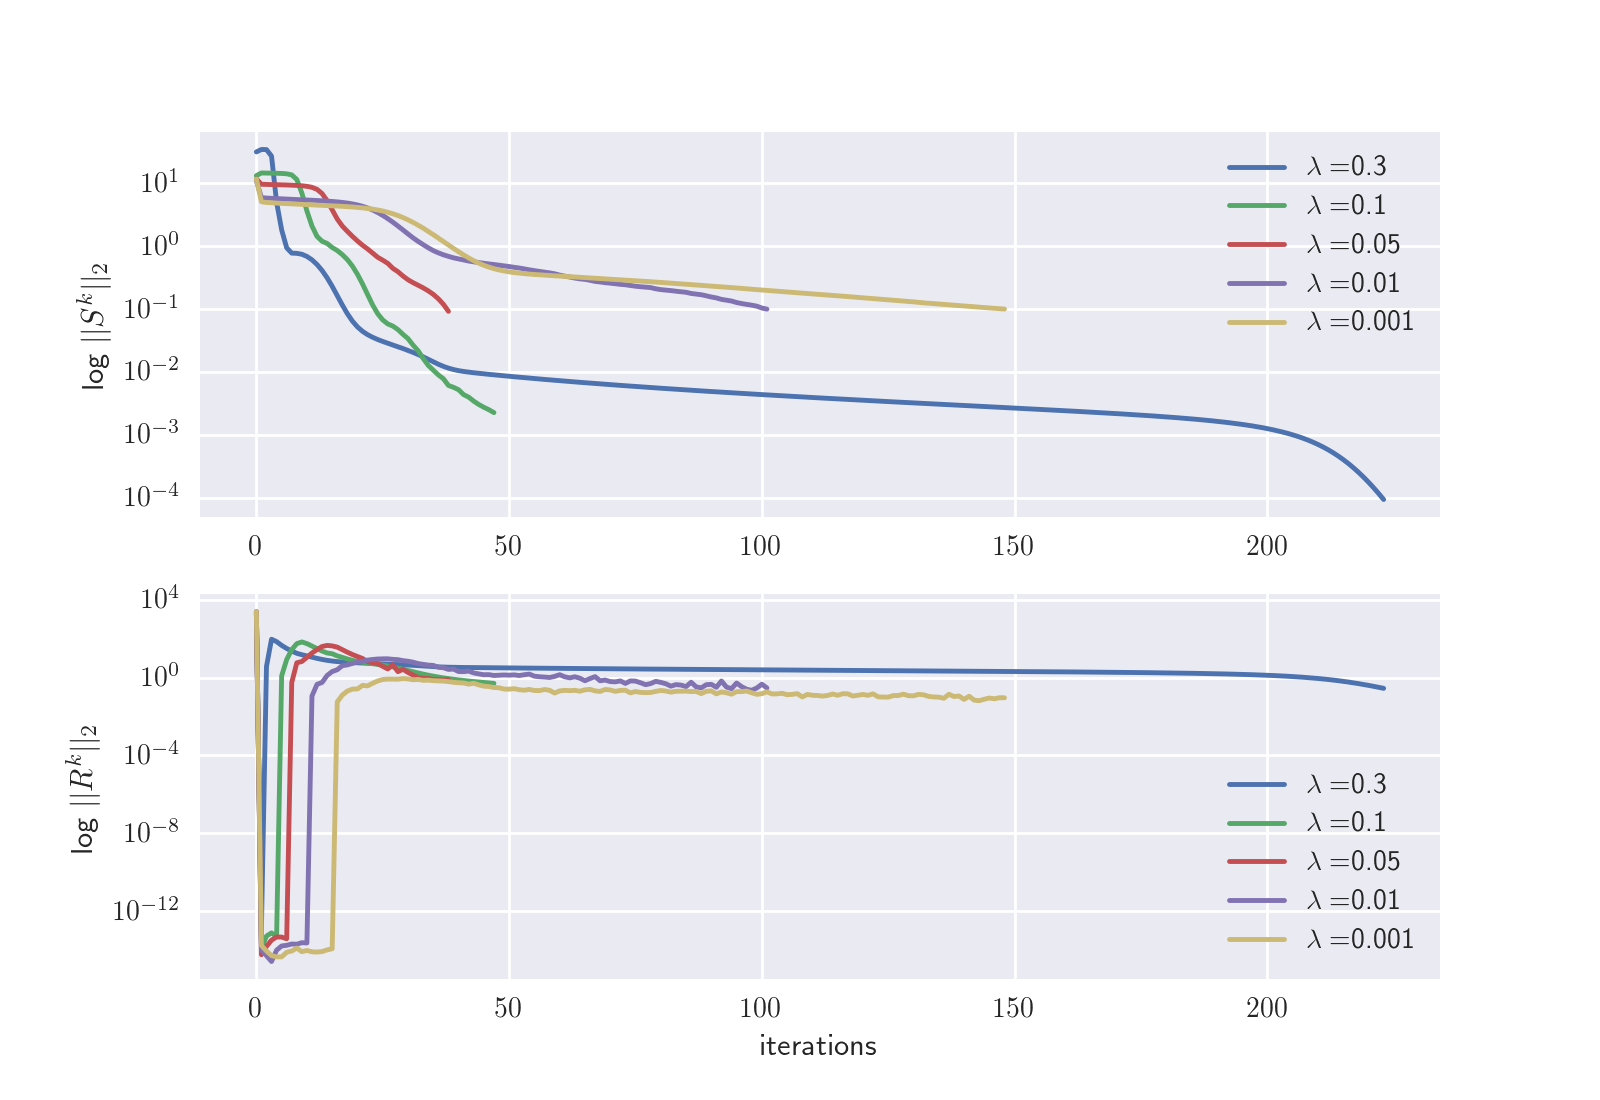
\includegraphics[width=\textwidth]{figures/convergence_lambda.png}
	\caption{Primal and Dual residuals convergence against $\lambda$ for fixed $\rho$}
	\label{fig:convlambda}
\end{figure}

The learning parameter, $\rho$, does not have impact on the accuracy of the solution but on the convergence speed. High values will decrease the dual function faster but the penalty for breaking primal feasibility will be high. In the figure \ref{fig:rhoiter}  we can see that the optimal point for $\lambda = 0.02$ is around 0.012.

\begin{figure}[H]
	\centering
	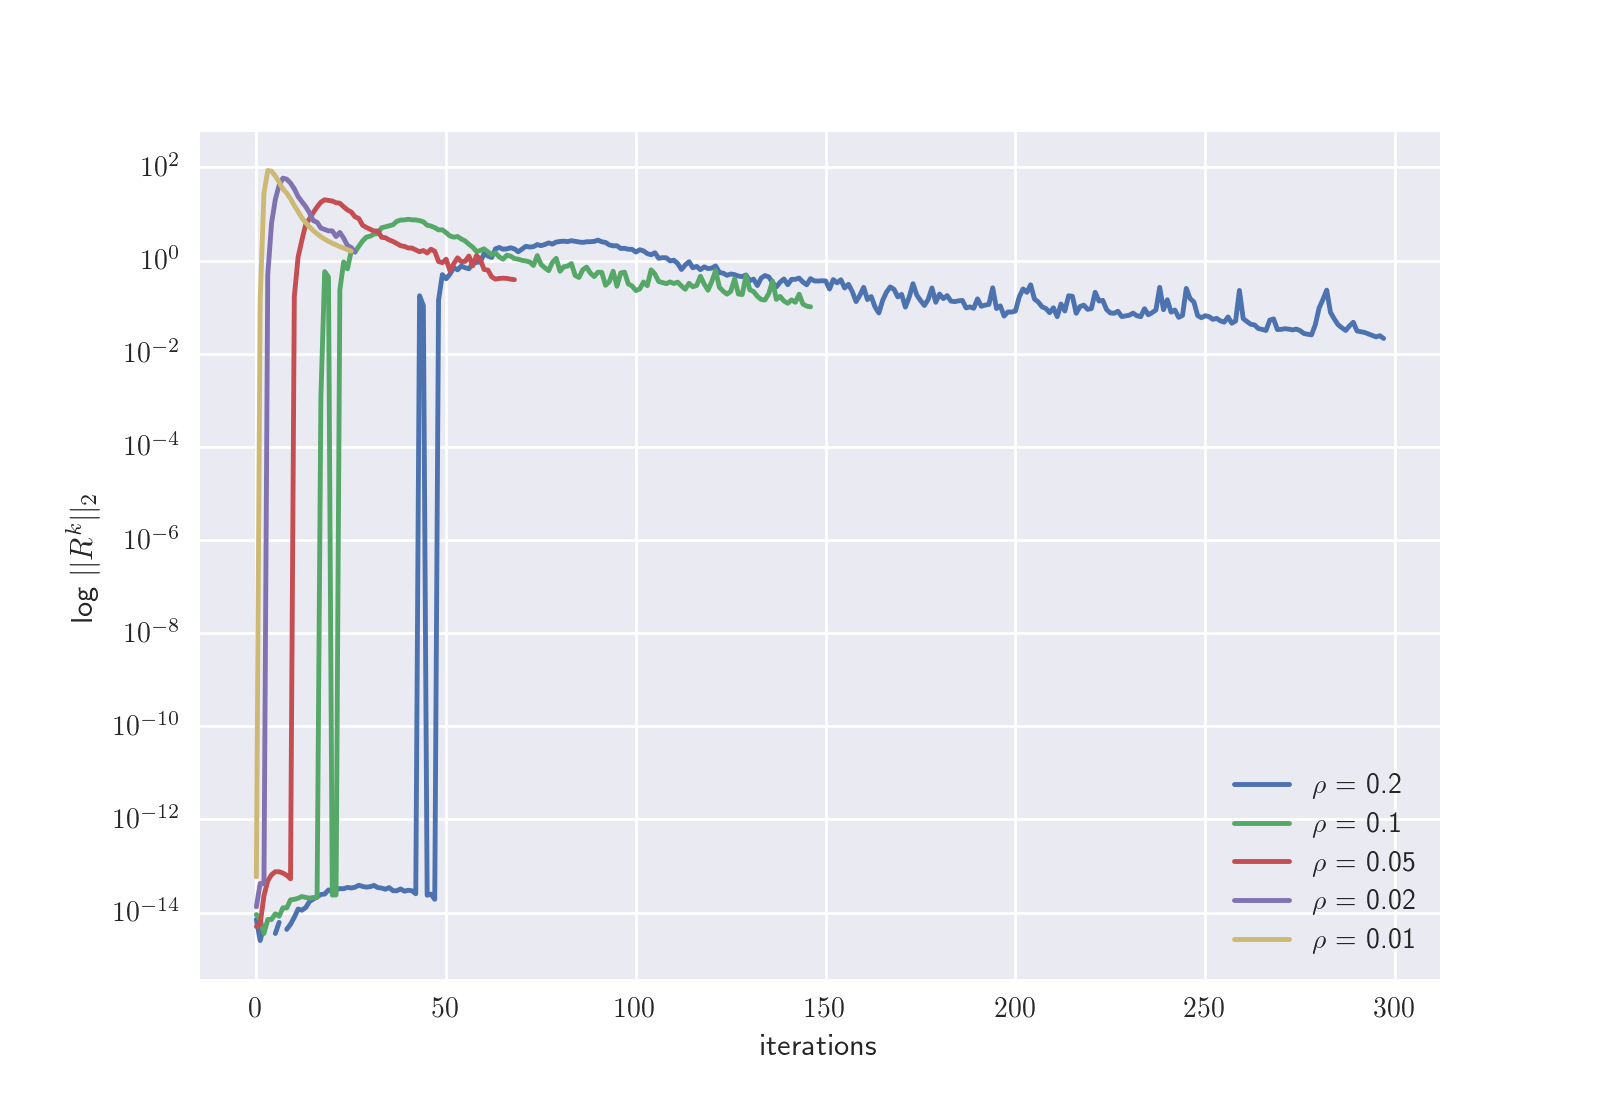
\includegraphics[width=\textwidth]{figures/convergence_rho.png}
	\caption{Primal residuals convergence against $\rho$ for $\lambda = 0.02$}
	\label{fig:convrho}
\end{figure}


\begin{figure}[H]
	\centering
	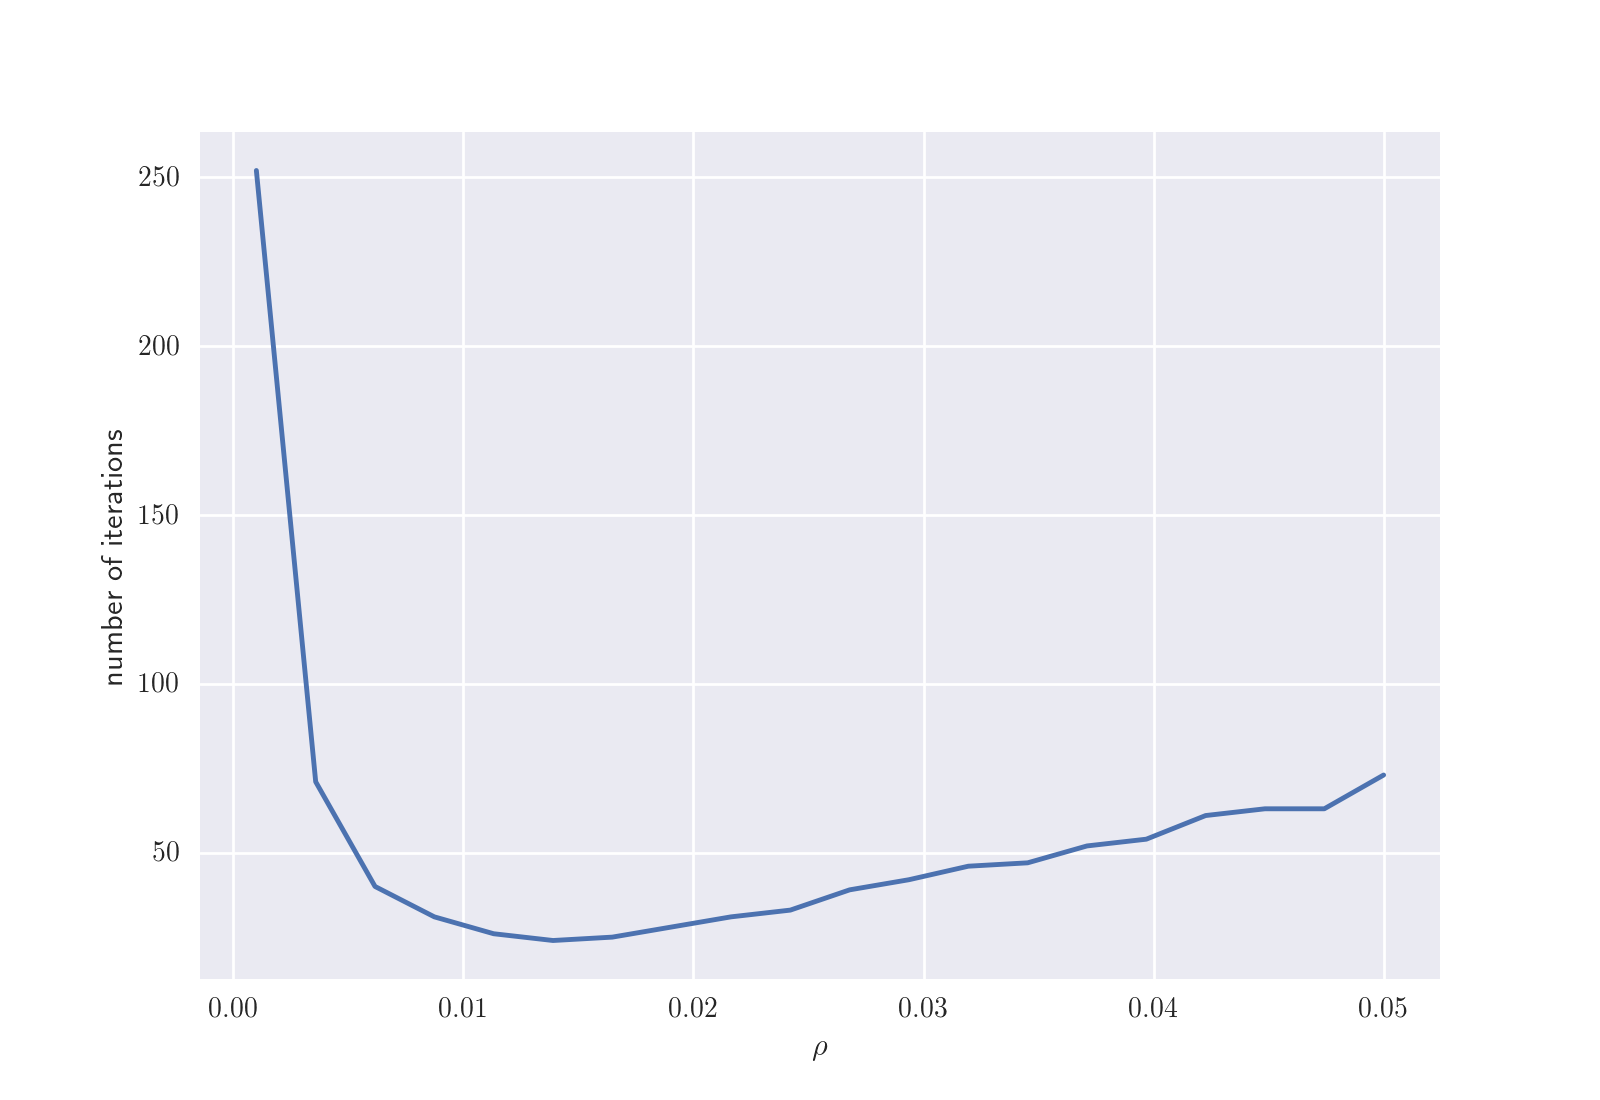
\includegraphics[width=\textwidth]{figures/rho_iter.png}
	\caption{Number of iterations against  $\rho$ for $\lambda = 0.02$}
	\label{fig:rhoiters}
\end{figure}

\section{Annex}

Proof of dual tolerance for (\ref{eq:admm_problem}). By optimality conditions we know that $\nabla_x L(X,Z^{k},U^{k}) = 0$. Hence,
\begin{align*}
0 &= C^T - (X^{k+1})^{-T} + \rho(X^{k+1}-Z^k+U^k) \\
 &= C^T - (X^{k+1})^{-T} + \rho(X^{k+1}-Z^k+U^k)+\rho Z^{k+1}-\rho Z^{k+1}  \\
&= C^T - (X^{k+1})^{-T} + \rho(R^{k+1}+U^k)+\rho (Z^{k+1}-Z^{k}) \\
&= C^T - (X^{k+1})^{-T} + \rho U^{k+1}+\rho (Z^{k+1}-Z^{k}) \\
\rho(Z^{k+1}-Z^{k})&= C^T - (X^{k+1})^{-T} + \rho U^{k+1}  \\
\rho S^{k+1}&= C^T - (X^{k+1})^{-T} + \rho U^{k+1}  \\
\end{align*}
which demonstrate the choice of (\ref{eq:ep_dual}).






\bibliographystyle{unsrt}
\bibliography{bibliography} 

\end{document}